\section{Overview per block}
\label{overview}

\subsection{Map generation}\label{Map generation}
The game will be played on a map that consists of a 9 by 9 grid that is surrounded by walls, resulting in a 11 x 11 field. There are also 16 walls within the playing field, which do not change during the course of the game. This results in a total of 65 playable spaces on which players walk and destructible crates or blocks can be placed, as shown in Fig. \ref{fig:layout}. The location of the crates is predetermined, but can be programmed to be randomized if time allows. At the start of the game players 1 and 2 are placed in the top left and bottom right corner respectively. The data of the grid is used as input in the block: Coordinates in section \ref{Coordinates}. This way every tile has a binary value for whether or not there is a crate present, based on this the right output can be determined in the coordinates block. The map generation is where this layout is defined.

\begin{figure}[H]
    \centering
    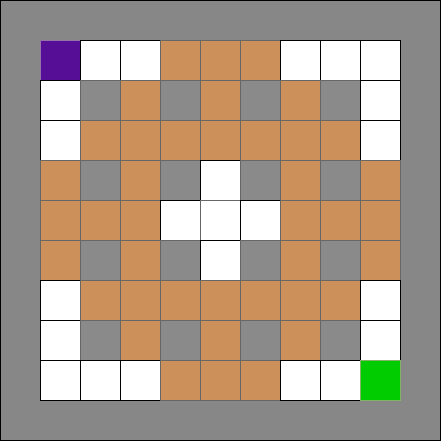
\includegraphics[width=0.4\textwidth]{Figures/bomberman.png}
    \caption{The layout of the bomberman grid, in which grey stands for walls, brown for crates, white the empty tiles and the remaining colours for the players.}
    \label{fig:layout}
\end{figure}


\subsection{Hitbox scanner}\label{Hitbox Scanner}
Another part of the design is how the player is able to move. The movement is based on the current position of the player and the inputs that are given. The players' locations are stored in two dimensional coordinates. The players are not allowed to walk towards spaces that contain either walls, crates or bombs. When the player places a bomb, it appears at the spot the player is currently at. The player should be able to move away from this spot. Furthermore, the player should be limited on how fast they can give inputs. Therefore a system has to be developed that makes sure the system waits for a certain duration before it becomes sensitive for the user's inputs again. This makes sure both players have the ability to move at the same speed. 

\subsection{Coordinates}\label{Coordinates}
The Coordinates block will send bomb location and players locations as output to the Hit Register and the Victory block. The generated map (\ref{Map generation} and the bomb timing signals \ref{BombTimer} are essential inputs of the Coordinates entity. Moreover, the player coordinates and bomb location are  important input.

Three distinct components are present at the output of the Coordinates block. Firstly, a propagated map. This map is merely subject to graphical changes, it forms the fundamental graphic layer presented on the screen. Another output makes sure the bombs are visible at the correct tiles at the appropriate times, overlapping the map. To achieve this, player positions and bomb timing signals will be used. Lastly, the player positions will be propagated.


%As for the inputs of Coordinates: Firstly the map generator will send the default layout shown in Fig. \ref{fig:layout}, from which the tile type and tile location together with both players starting points will be stored. After which the desired location for the movement and/or bomb placement from both players will be taken as input. Lastly, the Bomb Timer is the final input. The coordinates of the detonated bombs are important for the win condition.
 
 The coordinates of the bombs will be implemented using two 4-bit coordinates (\texttt{x} and \texttt{y}), the same goes for the player positions. This method is beneficial, because these elements are relatively scarce.
 %and active throughout gameplay (bombs explode with a certain tile radius, players move from tile to tile). The \texttt{x} and \texttt{y} values can be used efficiently to model these actions in VHDL.
 For the crates: each tile is represented by a flip flop, which can either contain a logic \texttt{'1'} (crate present on tile) or \texttt{'0'} (crate absent on tile). The walls will be hard coded as a logic \texttt{'1'} (wall present on tile) or \texttt{'0'} (wall absent on tile).
 
 \subsection{Bomb Timer}\label{BombTimer}
 Every bomb on the field needs their own timer. This timer is there to give the player time to move away from the bomb when it gets placed. Because timers usually require a large amount of flip-flops, some precautionary measures have to be taken: The timers will use the clock signal that will get generated for the VGA output, this will significantly reduce the amount of flip-flops necessary, these timers will also get reused by the Hit Register. When a bomb has been placed, the first timer of the Bomb timer will then start running. If another bomb gets placed, the Bomb timer will recognize that the first timer is in use and switch to the second timer. This will ensure that all bomb timers will run independently from each other.
 
 \subsection{Hit Register}
 When a bomb detonates, the bomb has a sort of radius in which it is checked if a player (or box in later iterations) is present. This is not a round like radius, but a horizontal and vertical line, in which everybody who is present (even the player who placed the bomb) loses the game or a life in later iterations. The first thing that is checked, is whether the exploding bomb has any hard walls next to it. %In the case that there is no wall present right next to the bomb, there will be no wall further than that unless it is the wall which blocks off the edge of the map. This needs to be done only once. If there is a wall above the bomb, than there must be a wall below the bomb. This is also the case with left and right. After that, 2 tiles on each side of the bomb will be checked on players or destructible crates.
 Then it will check if there are any players or crates inside the radius without going through a wall, meaning that the explosion cannot go through walls. A crate will be destroyed if it is detected. If a player gets detected, a signal will be sent to the Victory block.

\subsection{Victory}
This block can be seen as a multiplexer, where in a normal situation (nobody got hit) the output of coordinates is passed on to the output block and Hitbox scanner. In the case that somebody does get hit by a bomb, a victory screen will be passed on to the output. 
 
 \subsection{Output}\label{Output}
 To actually play the game it has to be displayed on a monitor. This will be done by using the VGA protocol. Although a VGA connector consists of 15 pins, only 5 of these will be used for the game. Three pins are needed to determine the colour of a specific pixel which is determined by the other two pins. Each of the three pins for the colour corresponds to a different colour, so for the colours red, green and blue. Each one can be set to off or on. Combinations of red, green and blue can make other colours. Therefore in total $2^3 = 8$ colours can be generated. Each pixel on the screen has to be coloured separately, this happens on the rising clock edge. The screen consists of 640x480 pixels. The refresh rate should be 60 Hz. There is also some time required to change from row and to start a new frame (with the two other pins). So in total a clock frequency of 25.175 MHz is required. Since the clock frequency of the chip is just 12.5 MHz, the resolution will be lower. This is in the case of this game not a very big issue. 
 The output module receives all the information of the coordinates from the coordinates module. This module should use this information to display the players, bombs, crates and the entire grid on the right pixel locations. Also sound effects can be added later on when for example a bomb detonates. 